% !TEX root = main.tex

\section{简介}

\subsection{实验目的}
\begin{itemize}
    \item 加深对计算机中整数及浮点数的位级表示的理解.
    \item 掌握C语言中位运算符的使用, 学会通过位操作来高效实现某些功能.
\end{itemize}
\subsection{实验要求}

使用规定的运算符, 在一定的操作数内实现以下逻辑与算术函数:

\begin{table}[H]
    \centering
    \footnotesize
    \begin{tabular}{llcc}
        \toprule
        Name & Description & Rating & Max ops \\
        \midrule
        \verb|bitXor(x,y)| & x || y using only \verb|&| and \verb|~|. & 1 & 14 \\
        \verb|tmin()| & Smallest two’s complement integer. & 1 & 4 \\
        \verb|isTmax(x)| & True only if \verb|x| is largest two's comp. integer. & 1 & 10 \\
        \verb|allOddBits(x)| & True only if all odd-numbered bits in \verb|x| set to 1. & 2 & 12 \\
        \verb|negate(x)| & Return \verb|-x| with using \verb|-| operator. & 2 & 5 \\
        \verb|isAsciDigit(x)| & True if \verb|0x30| $\leq$ \verb|x| $\leq$ \verb|0x39|. & 3 & 15 \\
        \verb|conditional| & Same as \verb|x?y:z| & 3 & 16 \\
        \verb|isLessOrEqual(x,y)| & True if \verb|x| $\leq$ \verb|y|, false otherwise. & 3 & 24 \\
        \verb|logicalNeg(x))| & Compute \verb|!x| without using \verb|!| operator. & 4 & 12 \\
        \verb|howManyBits(x)| & Min. no. of bits to represent \verb|x| in two’s comp. & 4 & 90 \\
        \verb|floatScale2(uf)| & Return bit-level equiv. of \verb|2*f| for f.p. arg. \verb|f|. & 4 & 30 \\
        \verb|floatFloat2Int(uf)| & Return bit-level equiv. of \verb|(int)f| for f.p. arg. \verb|f|. & 4 & 30 \\
        \verb|floatPower2(x)| & Return bit-level equiv. of \verb|2.0^x| for integer \verb|x|. & 4 & 30 \\
        \bottomrule
    \end{tabular}
    \caption{实验所给问题}
\end{table}

对于前10个整数问题, 代码中不允许出现超过8位的常数. 对于后3个浮点数问题, 允许出现 \verb|if| 等逻辑控制. 每个问题的具体限制, 参见\nameref{procedure}中各小题代码的注释. 

程序编写完毕后, 用测试程序 \verb|btest| 检查程序功能的正确性, 并用调整过的ANSI C编译器 \verb|dlc| 检查代码的合法性. 也可用Perl脚本 \verb|driver.pl| 进行综合评定. 

\subsection{实验环境}

本实验所有程序均在以下环境编译并通过测试:

\begin{table}[H]
    \centering
    \small
    \begin{tabular}{ll}
        Machine & MacBook Pro 13" \\
        SoC & Apple M1, 基于ARM, 含8核CPU、8核GPU及16GB RAM \\
        OS & macOS Monterey 12.3.1 \\
        IDE & Visual Studio Code 1.65.2 \\
        Docker & Docker 20.10.13 \\
        Image & Ubuntu 20.04.4, x86-64平台, 详见\nameref{env}部分 \\
        Packages & GCC 9.4.0, Make 4.2.1, Perl 5.30.0
    \end{tabular}
\end{table}

\section{实验结果}

依据要求完成 \verb|bits.c| 文件(见\nameref{codelist}) 并修改 \verb|Makefile| (见\nameref{env}), 在VS Code远程容器终端中运行 \verb|driver.pl|, 得到结果如下图所示:

\begin{figure}[H]
    \centering
    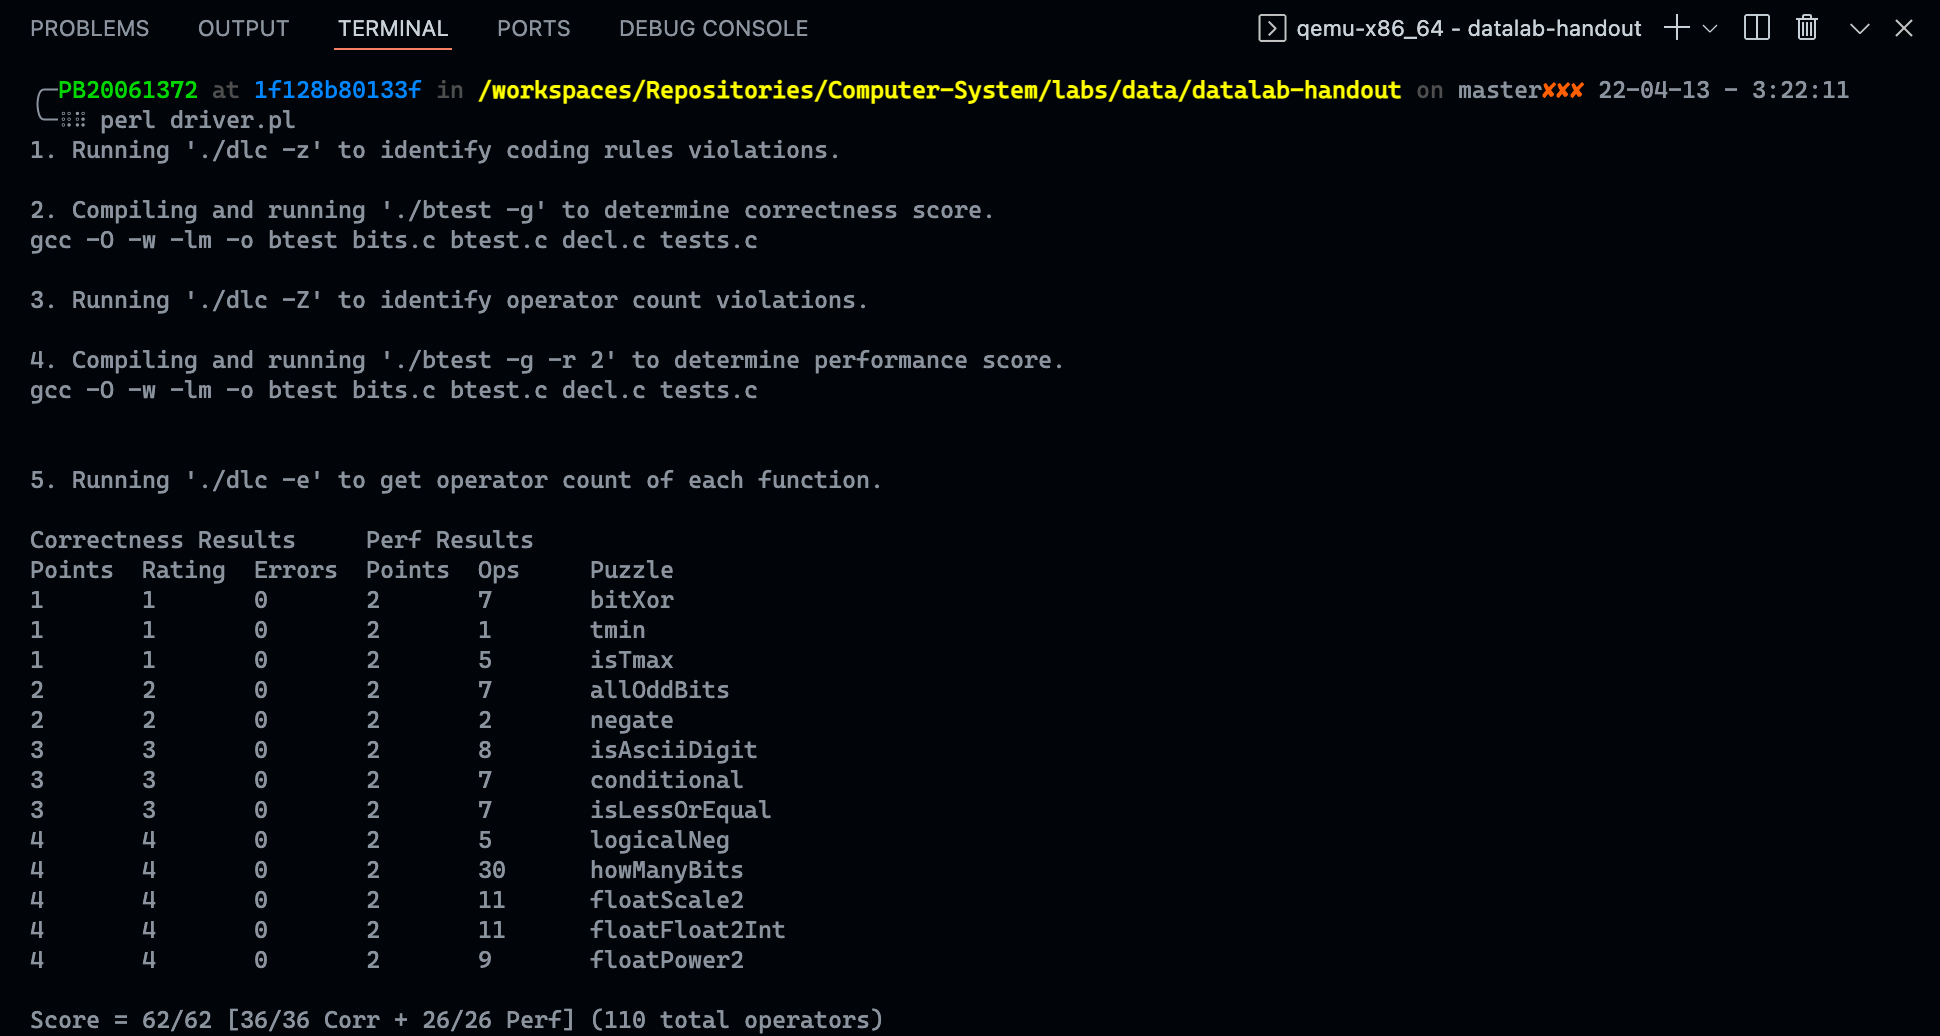
\includegraphics[width=\textwidth]{output.png}
    \cprotect\caption{\verb|driver.pl| 运行结果}
\end{figure}

可见, 程序的评估结果为满分, 正确性及性能均符合要求.

\section{实现思路}\label{procedure}

\subsection{\texttt{bitXor}}

本小题要求用位非和位与实现位异或. 对任意逻辑变量$A$和$B$, 根据异或运算的定义, 有
$$A \oplus B = (A+B)(AB)' $$
应用摩根律, 得
$$A \oplus B = (A'B')'(AB)' $$
使用C语言位运算符表达即可. 代码如下:
\begin{code}{c}
/*
 * bitXor - x^y using only ~ and &
 *   Example: bitXor(4, 5) = 1
 *   Legal ops: ~ &
 *   Max ops: 14
 *   Rating: 1
 */
int bitXor(int x, int y) { return ~(x & y) & ~(~x & ~y); }
\end{code}

根据评测结果, 该函数功能正确, 共计使用7个运算符.

\subsection{\texttt{tmin}}

本小题要求返回用补码表示的32位有符号整数的最小值. 根据补码的定义, 有符号整数的最小值仅有符号位为1, 其余位为0, 答案应为 \verb|0x8000|. 由于实验对常数大小的限制, 使用左移运算得到该值. 代码如下:

\begin{code}{c}
/*
 * tmin - return minimum two's complement integer
 *   Legal ops: ! ~ & ^ | + << >>
 *   Max ops: 4
 *   Rating: 1
 */
int tmin(void) { return 1 << 31; }
\end{code}

根据评测结果, 该函数功能正确, 仅使用1个运算符.

\subsection{\texttt{isTmax}}

本小题要求判断一个数是否为有符号整数的最大值, 返回值相当于 \verb|x==0x7FFFFFFF| 或 \verb|!(x^0x7FFFFFFF)|. 然而, 由于常数和运算符的限制, 应当利用该整数特有的运算性质来间接判断. 

经过简单观察, 发现该整数的反码恰等于其原码加一, 即 \verb|~x==x+1|, 或 \verb|!(~x^(x+1))|. 然而, \verb|0xFFFFFFFF| 也满足此运算性质, 需要根据 \verb|x+1!=0|, 或 \verb|!!(x+1)| 来排除. (此处连续使用2个逻辑非, 是为了将任意非零值变换为 \verb|0x1|, 下文涉及相同策略时不再特别指出.)

继续观察, 发现 \verb|x+1| 在以上操作中反复出现, 因而仍有优化空间——可以考虑将 \verb|x+1| 赋值给某个变量, 以便后续使用. 事实上, 对以上运算性质进一步思考, 发现该等式可以变换为 \verb|0xFFFFFFFF-x==x+1|, 或 \verb|(x+1)+(x+1)==0x0|, 从而充分利用 \verb|x+1|. 综合上述讨论, 并运用摩根律, 得到如下代码: 



\begin{code}{c}
/*
 * isTmax - returns 1 if x is the maximum, two's complement number,
 *     and 0 otherwise
 *   Legal ops: ! ~ & ^ | +
 *   Max ops: 10
 *   Rating: 1
 */
int isTmax(int x) {
  x = x + 1;
  return !(!x | (x + x));
}
\end{code}

根据评测结果, 该函数功能正确, 共计使用5个运算符.

\subsection{\texttt{allOddBits}}

本小题要求判断一个32位二进制字的奇数位是否全为1. 一种直接的思路是借助位掩码来判断, 记 \verb|mask=0x55555555|, 那么 \verb|x&mask==mask|, 或者说 \verb|!(~x&~mask)|. 然而, 由于常数大小的限制, 无法直接赋值上述 \verb|mask| 或 \verb|~mask|.

存在两种解决方案, 一是通过移位和位或运算生成该位掩码, 二是通过移位和位与运算合并 \verb|x| 的奇数位, 从而可用更短的位掩码 \verb|0xAA| 来判断. 笔者采用第二种方案, 代码如下:

\begin{code}{c}
/*
 * allOddBits - return 1 if all odd-numbered bits in word set to 1
 *   where bits are numbered from 0 (least significant) to 31 (most significant)
 *   Examples allOddBits(0xFFFFFFFD) = 0, allOddBits(0xAAAAAAAA) = 1
 *   Legal ops: ! ~ & ^ | + << >>
 *   Max ops: 12
 *   Rating: 2
 */
int allOddBits(int x) {
  x = x & x >> 16;
  return !(~(x & x >> 8) & 170);
}
\end{code}

根据评测结果, 该函数功能正确, 共计使用7个运算符.

\subsection{\texttt{negate}}

本小题要求对一个整数取反, 即求其补码. 根据定义有 \verb|-x==~x+1|. 代码如下:

\begin{code}{c}
/*
 * negate - return -x
 *   Example: negate(1) = -1.
 *   Legal ops: ! ~ & ^ | + << >>
 *   Max ops: 5
 *   Rating: 2
 */
int negate(int x) { return ~x + 1; }
\end{code}

根据评测结果, 该函数功能正确, 共计使用2个运算符.

\subsection{\texttt{isAsciiDigit}}

本小题要判断一个ASCII字符是否为数字0\textasciitilde9, 即 \verb|0x30<=x<=0x39|. 考虑 \verb|x-0x30| 和 \verb|x-0x3A| 的符号位, 应有 \verb|x-0x30>>31==0x0| 和  \verb|x-0x3A>>31==0x-1|. 此处, 应当注意右移运算扩展有符号数最高位的方式. 对常数取反进行优化, 有 \verb|(x+~57&~(x+~47))>>31==0x-1|. 合法的返回值应是上述表达式的最低位, 只需与 \verb|0x1| 做位与运算. 代码如下:

\begin{code}{c}
/*
 * isAsciiDigit - return 1 if 0x30 <= x <= 0x39 (ASCII codes for characters '0'
 * to '9') Example: isAsciiDigit(0x35) = 1. isAsciiDigit(0x3a) = 0.
 *            isAsciiDigit(0x05) = 0.
 *   Legal ops: ! ~ & ^ | + << >>
 *   Max ops: 15
 *   Rating: 3
 */
int isAsciiDigit(int x) { return (x + ~57 & ~(x + ~47)) >> 31 & 1; }
\end{code}

根据评测结果, 该函数功能正确, 共计使用8个运算符.

\subsection{\texttt{conditional}}

本小题要求用位运算实现三目运算符, 可以抽象为2选1数据选择器. 考虑到记号的简洁性, 不妨设地址信号$X$、输入数据$Y,Z$和输出数据$D$均为一维逻辑变量, 则有
$$D=XY+X'Z$$

要对位向量 \verb|x,y,z| 的每一位进行上述操作, 应将任意非零值 \verb|x| 统一变换为 \verb|0xFFFFFFFF|. 可以先通过逻辑非运算将取值限定为0或1, 再减去1得到预期的变换结果, 即 \verb|x=!x+~0|. 代码如下:

\begin{code}{c}
/*
 * conditional - same as x ? y : z
 *   Example: conditional(2,4,5) = 4
 *   Legal ops: ! ~ & ^ | + << >>
 *   Max ops: 16
 *   Rating: 3
 */
int conditional(int x, int y, int z) {
  x = !x + ~0;
  return (x & y) | (~x & z);
}
\end{code}

根据评测结果, 该函数功能正确, 共计使用7个运算符.

\subsection{\texttt{isLessOrEqual}}

本小题要求比较两个有符号整数的大小, 返回 \verb|x<=y|. 由于补码运算的溢出问题, 或者说由于模$2^{32}$整数加群的结构, 不能简单通过 \verb|y-x| 的符号位来判断. 

对模$2^{32}$剩余类进行分析, 发现可能存在两种错误情况: 一是 \verb|x| 为正整数, \verb|y| 为负整数, 但 \verb|y-x| 为正整数;  二是 \verb|x| 为负整数, \verb|y| 为非负整数, 但 \verb|y-x| 为负整数. 应当在 \verb|x| 和 \verb|y| 符号相反时采用其他判断方法——显然, 只需返回 \verb|x| 的符号位.

综上所述, 当 \verb|(x^y)>>31==0x-1| (符号相反)时, 返回 \verb|x| 的符号位; 当 \verb|(x^y)>>31==0x0| (符号相同)时, 返回 \verb|y-x| 的符号位取反, 或者直接返回 \verb|x-y-1| (即\verb|x+~y|)的符号位. 

能否将两种情况合为一个表达式? 答案是肯定的, 只需将 \verb|~((x^y)>>31)| 作为位掩码, 用于决定是否将 \verb|x| 加上 \verb|~y|. 进一步利用摩根律, 得到最终代码如下:

\begin{code}{c}
/*
 * isLessOrEqual - if x <= y  then return 1, else return 0
 *   Example: isLessOrEqual(4,5) = 1.
 *   Legal ops: ! ~ & ^ | + << >>
 *   Max ops: 24
 *   Rating: 3
 */
int isLessOrEqual(int x, int y) { return (x + ~((x ^ y) >> 31 | y)) >> 31 & 1; }
\end{code}

根据评测结果, 该函数功能正确, 共计使用7个运算符.

\subsection{\texttt{logicalNeg}}

本小题要求用位运算实现逻辑非: 将任意非零值映射为0, 而将0映射为1. 相较于0, 非零整数的特征在于其自身和相反数必有一个符号位为1. 遵循这个思路, 再借助右移运算, 可将任意非零值映射为 \verb|0xFFFFFFFF| , 加上1便得到预期返回值. 代码如下:

\begin{code}{c}
/*
 * logicalNeg - implement the ! operator, using all of
 *              the legal operators except !
 *   Examples: logicalNeg(3) = 0, logicalNeg(0) = 1
 *   Legal ops: ~ & ^ | + << >>
 *   Max ops: 12
 *   Rating: 4
 */
int logicalNeg(int x) { return ((x | (~x + 1)) >> 31) + 1; }
\end{code}

根据评测结果, 该函数功能正确, 共计使用5个运算符.

\subsection{\texttt{howManyBits}}

本小题要求返回用补码表示某个整数需要的最少二进制位数. 由于该整数已由32位补码给出, 经分析, 需进行如下处理: 

对于符号位为0的非负整数, 找到最高位的1所在位置; 对于符号位为1的负整数, 找到最高位的0所在位置. 取该位置之后的所有位并加上符号位, 就是表示该整数的最短补码.

为了统一上述两种情况而节省操作数, 首先将 \verb|x| 赋值为 \verb|x>>31^x|, 使得负数取反, 非负数保持不变. 然后, 采用分治策略查找最高位的1: 

\begin{enumerate}[noitemsep]
    \item 若 \verb|x| 的高16位有1 (即\verb|!!(x>>16)|), 则将 \verb|x| 右移16位, 在高16位继续查找; 否则, 在低16位继续查找. 
    \item 将 \verb|x| 视作16位补码, 若 \verb|x| 的高8位有1 (即\verb|!!(x>>8)|), 则将 \verb|x| 右移8位, 在高8位继续查找; 否则, 在低8位继续查找. 
    \item 将 \verb|x| 视作8位补码, 依此类推, 直到找到最高位的1或找不到1.
\end{enumerate}

上述分治过程为计算最高位1的位置提供了便利. 记最高位1的位置为  \verb|sum|, 考虑其二进制表示, 每当 \verb|x| 右移$2^i$位 ($i=4,3,2,1,0$), 将 \verb|sum| 加上$2^i$. 若最后 \verb|x| 为0, 说明找不到为1的位, 函数返回 \verb|sum + 1|; 若最后 \verb|x| 为1, 返回  \verb|sum + 2|.

完整代码如下:  

\begin{code}{c}
/* howManyBits - return the minimum number of bits required to represent x in
 *             two's complement
 *  Examples: howManyBits(12) = 5
 *            howManyBits(298) = 10
 *            howManyBits(-5) = 4
 *            howManyBits(0)  = 1
 *            howManyBits(-1) = 1
 *            howManyBits(0x80000000) = 32
 *  Legal ops: ! ~ & ^ | + << >>
 *  Max ops: 90
 *  Rating: 4
 */
int howManyBits(int x) {
  int sum, tmp;
  x = x >> 31 ^ x;
  sum = !!(x >> 16) << 4, x = x >> sum;
  tmp = !!(x >> 8) << 3, sum = sum + tmp, x = x >> tmp;
  tmp = !!(x >> 4) << 2, sum = sum + tmp, x = x >> tmp;
  tmp = !!(x >> 2) << 1, sum = sum + tmp, x = x >> tmp;
  tmp = x >> 1, sum = sum + tmp, x = x >> tmp;
  return sum + x + 1;
}
\end{code}

根据评测结果, 该函数功能正确, 共计使用30个运算符.

\subsection{\texttt{floatScale2}}

本小题以无符号整数 \verb|uf| 的形式给出一个IEEE标准的32位浮点数 \verb|f|, 要求返回 \verb|2*f|. 为使程序逻辑清晰, 首先利用位掩码将该浮点数拆分为符号位 \verb|s|, 阶数部分 \verb|e|, 以及尾数部分 \verb|f|, 进而分类讨论:

\begin{enumerate}[noitemsep]
    \item 若阶数为0, 为非规格数, 乘2相当于将尾数部分左移1位. 经检验, 该操作能够兼顾乘2后非规格数变为规格数(阶数加1)的情况. 返回 \verb#s|m<<1#.
    \item 若阶数为254, 乘2后为无穷, 应将尾数置零并继续下一步.
    \item 若阶数为255, 为 \verb|NaN| 或无穷, 返回原值; 否则将阶数加1后返回 \verb#s|e|m#.
\end{enumerate}

完整代码如下:

\begin{code}{c}
/*
 * floatScale2 - Return bit-level equivalent of expression 2*f for
 *   floating point argument f.
 *   Both the argument and result are passed as unsigned int's, but
 *   they are to be interpreted as the bit-level representation of
 *   single-precision floating point values.
 *   When argument is NaN, return argument
 *   Legal ops: Any integer/unsigned operations incl. ||, &&. also if, while
 *   Max ops: 30
 *   Rating: 4
 */
unsigned floatScale2(unsigned uf) {
  int s = uf & 0x80000000;
  int e = uf & 0x7F800000;
  int m = uf & 0x007FFFFF;
  if (!e)
    return s | m << 1;
  if (e == 0x7F000000)
    m = 0;
  if (e != 0x7F800000)
    e += 0x00800000;
  return s | e | m;
}
\end{code}

根据评测结果, 该函数功能正确, 共计使用11个运算符.

\subsection{\texttt{floatFloat2Int}}

本小题要求实现浮点数向整数的类型转换. 同样, 为使程序逻辑清晰, 首先利用位掩码将该浮点数拆分为符号位 \verb|s|, 阶数部分 \verb|e|, 以及尾数部分 \verb|f|, 进而分类讨论:

\begin{enumerate}[noitemsep]
    \item 若阶数小于127, 偏移后指数小于0, 该浮点数仅有小数部分, 返回0.
    \item 若阶数大于157, 该浮点数超过32位整数范围, 溢出. 按注释要求, 返回 \verb|0x80000000|.
    \item 其他情况, 将尾数并上最高有效位1, 左移与符号位对齐, 最后将整体根据指数右移, 得到所求整数.
\end{enumerate}

完整代码如下:

\begin{code}{c}
/*
 * floatFloat2Int - Return bit-level equivalent of expression (int) f
 *   for floating point argument f.
 *   Argument is passed as unsigned int, but
 *   it is to be interpreted as the bit-level representation of a
 *   single-precision floating point value.
 *   Anything out of range (including NaN and infinity) should return
 *   0x80000000u.
 *   Legal ops: Any integer/unsigned operations incl. ||, &&. also if, while
 *   Max ops: 30
 *   Rating: 4
 */
int floatFloat2Int(unsigned uf) {
  int s = uf & 0x80000000;
  int e = (uf >> 23) & 0xFF;
  int m = uf & 0x007FFFFF;
  if (e < 127)
    return 0;
  if (e > 157)
    return 0x80000000;
  return (s | 0x40000000 | m << 7) >> 157 - e;
}
\end{code}

根据评测结果, 该函数功能正确, 共计使用11个运算符.

\subsection{\texttt{floatPower2}}

本小题要求用浮点数返回2的 \verb|x| 次幂. 分三种情况讨论:

\begin{enumerate}[noitemsep]
    \item 若 \verb|x>127|, 上溢, 返回正无穷(\verb|0x7F800000|).
    \item 若 \verb|x<=127&&x>=-126|, 为规格数, 偏移得阶数为 \verb|x+127|, 返回 \verb|x+127<<23|.
    \item 若 \verb|x<--126&&x>=-149|, 为非规格数, 仅尾数部分的第 \verb|149+x| 位为1, 返回 \verb|1<<149+x|.
    \item 若 \verb|x<-149|, 下溢, 返回0.
\end{enumerate}

完整代码如下:

\begin{code}{c}
/*
 * floatPower2 - Return bit-level equivalent of the expression 2.0^x
 *   (2.0 raised to the power x) for any 32-bit integer x.
 *
 *   The unsigned value that is returned should have the identical bit
 *   representation as the single-precision floating-point number 2.0^x.
 *   If the result is too small to be represented as a denorm, return
 *   0. If too large, return +INF.
 *
 *   Legal ops: Any integer/unsigned operations incl. ||, &&. Also if, while
 *   Max ops: 30
 *   Rating: 4
 */
unsigned floatPower2(int x) {
  if (x > 127)
    return 0x7F800000;
  if (x >= -126)
    return x + 127 << 23;
  if (x >= -149)
    return 1 << 149 + x;
  return 0;
}
\end{code}

根据评测结果, 该函数功能正确, 共计使用9个运算符.

\section{总结}

完成Data Lab, 主要有以下收获:

\begin{itemize}
    \item 加深了对计算机中整数和浮点数格式的理解, 尤其是浮点数运算的实现思路.
    \item 掌握了C语言位运算符的优先级关系和特性, 尤其是右移运算符补全高位的方式.
    \item 积累了位运算符的使用技巧, 如: 通过两次逻辑非将任意整数转换为布尔类型, 通过位掩码得到指定位的值等.
    \item 理解了镜像、容器等概念, 学会了Docker的使用, 能够编写简易的Dockerfile.
    \item 熟悉了Linux中常见软件包, 能够在终端中使用Linux常见命令.
\end{itemize}

本实验的所有材料及代码已上传至GitHub:

\url{https://github.com/HasiNed/Computer-System}

\setupappendix

\clearpage
\section{环境搭建}\label{env}

本实验涉及的部分二进制文件依赖于Linux/amd64环境以及相关软件包. 由于笔者的机器基于ARM指令集, 无法直接满足环境需求, 因而使用Docker仿真x86-64平台, 并搭建Ubuntu虚拟环境. 具体步骤如下:
\begin{enumerate}[noitemsep]
    \item 安装VS Code、Docker Desktop等应用, 此处从略.
    \item 编写Dockerfile (完整文件见\nameref{codelist}), 大意如下.
    
    \begin{itemize}
        \item 从Docker Hub引入Ubuntu官方镜像:
        
        \begin{restoreindent}
\begin{code}{dockerfile}
FROM --platform=linux/x86_64 ubuntu:latest
\end{code}
        \end{restoreindent}

        \item 安装build-essential, perl等软件包:
        
        \begin{restoreindent}
\begin{code}{dockerfile}
 RUN apt-get update \
    && apt-get -y install sudo git zsh vim perl curl locales build-essential \ 
    && apt-get clean -y
\end{code}
        \end{restoreindent}

        此处, 出于功能性考虑, 额外安装了sudo, zsh, vim等包.

        \item 创建non-root用户, 用于存放学号:
        
        \begin{restoreindent}
\begin{code}{dockerfile}
ARG USERNAME="PB20061372"
RUN useradd $USERNAME -m \
    && echo "$USERNAME ALL=(ALL) NOPASSWD: ALL" > /etc/sudoers.d/$USERNAME \
    && chmod 0440 /etc/sudoers.d/$USERNAME
USER $USERNAME
\end{code}
        \end{restoreindent}

        此处, 应当赋予新用户 \verb|sudo| 命令权限.

        \item 安装oh-my-zsh并个性化主题, 从而显示必要信息:

        \begin{restoreindent}
\begin{code}{dockerfile}
RUN sh -c "$(curl -fsSL https://raw.githubusercontent.com/ohmyzsh/ohmyzsh/master/tools/install.sh)" ""
RUN sed -i "s/robbyrussell/fino-time/g" ~/.zshrc
\end{code}
        \end{restoreindent}

    \end{itemize}

    \item 在VS Code中, 安装Remote - Containers插件. 在工作区中配置Dev Container, 用于自动生成容器以及切换工作环境.
    \item 在远程容器中打开工作路径并执行 \verb|uname -a| 命令, 应有如下格式输出: 
    
    \begin{figure}[H]
        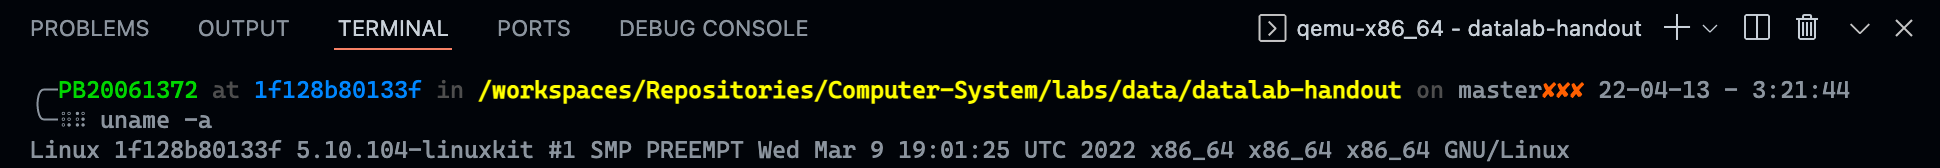
\includegraphics[width=\textwidth]{env.png}
        \caption{在远程容器中查看机器环境}
    \end{figure}
    
    \item 将所给的\verb|Makefile|文件中 \verb|CFLAGS = -O -Wall -m32| 修改为 \verb|CFLAGS = -O -w|, 从而编译64位程序, 避免安装交叉编译所需的额外软件包, 同时消除因编程风格导致的部分警告. 

\end{enumerate}

至此, 实验环境搭建完毕. \verb|bits.c|, \verb|ishow.c|, \verb|fshow.c|, \verb|btest.c|, \verb|dlc|, \verb|driver.pl| 等均可在Ubuntu容器中编译或运行.

\clearpage
\section{代码清单}\label{codelist}

\subsection[\texttt{bits.c}]{\texttt{bits.c}\footnote{出于篇幅考虑, 删除了大段注释.}}

\includecode{c}{bits.c}

\clearpage
\subsection{\texttt{Dockerfile}}

\includecode{dockerfile}{Dockerfile}